\documentclass{ximera}

 

\usepackage{epsfig}

\graphicspath{
  {./}
  {figures/}
}

\usepackage{morewrites}
\makeatletter
\newcommand\subfile[1]{%
\renewcommand{\input}[1]{}%
\begingroup\skip@preamble\otherinput{#1}\endgroup\par\vspace{\topsep}
\let\input\otherinput}
\makeatother

\newcommand{\includeexercises}{\directlua{dofile("/home/jim/linearAlgebra/laode/exercises.lua")}}

%\newcounter{ccounter}
%\setcounter{ccounter}{1}
%\newcommand{\Chapter}[1]{\setcounter{chapter}{\arabic{ccounter}}\chapter{#1}\addtocounter{ccounter}{1}}

%\newcommand{\section}[1]{\section{#1}\setcounter{thm}{0}\setcounter{equation}{0}}

%\renewcommand{\theequation}{\arabic{chapter}.\arabic{section}.\arabic{equation}}
%\renewcommand{\thefigure}{\arabic{chapter}.\arabic{figure}}
%\renewcommand{\thetable}{\arabic{chapter}.\arabic{table}}

%\newcommand{\Sec}[2]{\section{#1}\markright{\arabic{ccounter}.\arabic{section}.#2}\setcounter{equation}{0}\setcounter{thm}{0}\setcounter{figure}{0}}

\newcommand{\Sec}[2]{\section{#1}}

\setcounter{secnumdepth}{2}
%\setcounter{secnumdepth}{1} 

%\newcounter{THM}
%\renewcommand{\theTHM}{\arabic{chapter}.\arabic{section}}

\newcommand{\trademark}{{R\!\!\!\!\!\bigcirc}}
%\newtheorem{exercise}{}

\newcommand{\dfield}{{\sf dfield9}}
\newcommand{\pplane}{{\sf pplane9}}

\newcommand{\EXER}{\section*{Exercises}}%\vspace*{0.2in}\hrule\small\setcounter{exercise}{0}}
\newcommand{\CEXER}{}%\vspace{0.08in}\begin{center}Computer Exercises\end{center}}
\newcommand{\TEXER}{} %\vspace{0.08in}\begin{center}Hand Exercises\end{center}}
\newcommand{\AEXER}{} %\vspace{0.08in}\begin{center}Hand Exercises\end{center}}

% BADBAD: \newcommand{\Bbb}{\bf}

\newcommand{\R}{\mbox{$\Bbb{R}$}}
\newcommand{\C}{\mbox{$\Bbb{C}$}}
\newcommand{\Z}{\mbox{$\Bbb{Z}$}}
\newcommand{\N}{\mbox{$\Bbb{N}$}}
\newcommand{\D}{\mbox{{\bf D}}}
\usepackage{amssymb}
%\newcommand{\qed}{\hfill\mbox{\raggedright$\square$} \vspace{1ex}}
%\newcommand{\proof}{\noindent {\bf Proof:} \hspace{0.1in}}

\newcommand{\setmin}{\;\mbox{--}\;}
\newcommand{\Matlab}{{M\small{AT\-LAB}} }
\newcommand{\Matlabp}{{M\small{AT\-LAB}}}
\newcommand{\computer}{\Matlab Instructions}
\newcommand{\half}{\mbox{$\frac{1}{2}$}}
\newcommand{\compose}{\raisebox{.15ex}{\mbox{{\scriptsize$\circ$}}}}
\newcommand{\AND}{\quad\mbox{and}\quad}
\newcommand{\vect}[2]{\left(\begin{array}{c} #1_1 \\ \vdots \\
 #1_{#2}\end{array}\right)}
\newcommand{\mattwo}[4]{\left(\begin{array}{rr} #1 & #2\\ #3
&#4\end{array}\right)}
\newcommand{\mattwoc}[4]{\left(\begin{array}{cc} #1 & #2\\ #3
&#4\end{array}\right)}
\newcommand{\vectwo}[2]{\left(\begin{array}{r} #1 \\ #2\end{array}\right)}
\newcommand{\vectwoc}[2]{\left(\begin{array}{c} #1 \\ #2\end{array}\right)}

\newcommand{\ignore}[1]{}


\newcommand{\inv}{^{-1}}
\newcommand{\CC}{{\cal C}}
\newcommand{\CCone}{\CC^1}
\newcommand{\Span}{{\rm span}}
\newcommand{\rank}{{\rm rank}}
\newcommand{\trace}{{\rm tr}}
\newcommand{\RE}{{\rm Re}}
\newcommand{\IM}{{\rm Im}}
\newcommand{\nulls}{{\rm null\;space}}

\newcommand{\dps}{\displaystyle}
\newcommand{\arraystart}{\renewcommand{\arraystretch}{1.8}}
\newcommand{\arrayfinish}{\renewcommand{\arraystretch}{1.2}}
\newcommand{\Start}[1]{\vspace{0.08in}\noindent {\bf Section~\ref{#1}}}
\newcommand{\exer}[1]{\noindent {\bf \ref{#1}}}
\newcommand{\ans}{}
\newcommand{\matthree}[9]{\left(\begin{array}{rrr} #1 & #2 & #3 \\ #4 & #5 & #6
\\ #7 & #8 & #9\end{array}\right)}
\newcommand{\cvectwo}[2]{\left(\begin{array}{c} #1 \\ #2\end{array}\right)}
\newcommand{\cmatthree}[9]{\left(\begin{array}{ccc} #1 & #2 & #3 \\ #4 & #5 &
#6 \\ #7 & #8 & #9\end{array}\right)}
\newcommand{\vecthree}[3]{\left(\begin{array}{r} #1 \\ #2 \\
#3\end{array}\right)}
\newcommand{\cvecthree}[3]{\left(\begin{array}{c} #1 \\ #2 \\
#3\end{array}\right)}
\newcommand{\cmattwo}[4]{\left(\begin{array}{cc} #1 & #2\\ #3
&#4\end{array}\right)}

\newcommand{\Matrix}[1]{\ensuremath{\left(\begin{array}{rrrrrrrrrrrrrrrrrr} #1 \end{array}\right)}}

\newcommand{\Matrixc}[1]{\ensuremath{\left(\begin{array}{cccccccccccc} #1 \end{array}\right)}}



\renewcommand{\labelenumi}{\theenumi)}
\newenvironment{enumeratea}%
{\begingroup
 \renewcommand{\theenumi}{\alph{enumi}}
 \renewcommand{\labelenumi}{(\theenumi)}
 \begin{enumerate}}
 {\end{enumerate}\endgroup}



\newcounter{help}
\renewcommand{\thehelp}{\thesection.\arabic{equation}}

%\newenvironment{equation*}%
%{\renewcommand\endequation{\eqno (\theequation)* $$}%
%   \begin{equation}}%
%   {\end{equation}\renewcommand\endequation{\eqno \@eqnnum
%$$\global\@ignoretrue}}

%\input{psfig.tex}

\author{Martin Golubitsky and Michael Dellnitz}

%\newenvironment{matlabEquation}%
%{\renewcommand\endequation{\eqno (\theequation*) $$}%
%   \begin{equation}}%
%   {\end{equation}\renewcommand\endequation{\eqno \@eqnnum
% $$\global\@ignoretrue}}

\newcommand{\soln}{\textbf{Solution:} }
\newcommand{\exercap}[1]{\centerline{Figure~\ref{#1}}}
\newcommand{\exercaptwo}[1]{\centerline{Figure~\ref{#1}a\hspace{2.1in}
Figure~\ref{#1}b}}
\newcommand{\exercapthree}[1]{\centerline{Figure~\ref{#1}a\hspace{1.2in}
Figure~\ref{#1}b\hspace{1.2in}Figure~\ref{#1}c}}
\newcommand{\para}{\hspace{0.4in}}

\renewenvironment{solution}{\suppress}{\endsuppress}

\ifxake
\newenvironment{matlabEquation}{\begin{equation}}{\end{equation}}
\else
\newenvironment{matlabEquation}%
{\let\oldtheequation\theequation\renewcommand{\theequation}{\oldtheequation*}\begin{equation}}%
  {\end{equation}\let\theequation\oldtheequation}
\fi

\makeatother


\title{The Initial Value Problem}

\begin{document}
\begin{abstract}
\end{abstract}
\maketitle

 \index{initial value problem}
\label{S:6.1}

Recall that a planar autonomous \index{autonomous} system of
ordinary differential equations has the form
\arraystart
\begin{equation}  \label{2dsystem}
\begin{array}{ccl}
\dps \frac{dx}{dt}  & = & f(x,y) \\
\dps \frac{dy}{dt}  & = & g(x,y).
\end{array}
\end{equation}
\arrayfinish
Computer experiments using {\sf pplane5} always appear to find a unique
solution to initial value problems.  More precisely, we are led to
believe that there is just one solution to \Ref{2dsystem} satisfying
the initial conditions\index{initial condition}
\begin{eqnarray*}
x(0) & = & x_0 \\
y(0) & = & y_0.
\end{eqnarray*}

\subsection*{Existence and Uniqueness of Solutions}

In fact, existence \index{existence of solutions} and uniqueness
of solutions \index{uniqueness of solutions} are not always guaranteed
--- though they are guaranteed for a large class of differential
equations, as the following theorem shows.

\begin{theorem}  \label{exist&unique}
Suppose that the functions $f$ and $g$ in the system of
differential equations \Ref{2dsystem} are differentiable near
$(x_0,y_0)$ and that the partial derivatives $f_x,f_y,g_x,g_y$
are continuous near $(x_0,y_0)$.  Then there exists a unique
solution to \Ref{2dsystem} with initial conditions
$(x(0),y(0))=(x_0,y_0)$.
\end{theorem} \index{uniqueness of solutions}

For example, consider the planar system of constant coefficient linear
differential equations:
\arraystart
\begin{equation}  \label{2dlinsystem}
\begin{array}{ccl}
\dps \frac{dx}{dt}  & = & ax+by \\
\dps \frac{dy}{dt}  & = & cx+dy.
\end{array}
\end{equation}
\arrayfinish
In \Ref{2dlinsystem}, $f(x,y)=ax+by$ and $g(x,y)=cx+dy$.  The partial
derivatives of $f$ and $g$ are easy to calculate; they are: $f_x=a$, $f_y=b$,
$g_x=c$, and $g_y=d$.  As constant functions, all of these partial
derivatives are continuous.  Hence, existence and uniqueness of solutions to
the initial value problem for \Ref{2dlinsystem} are guaranteed by
Theorem~\ref{exist&unique}.


Although we have stated this theorem just for planar systems, the theorem
itself is valid in all dimensions.   For example, in one dimension the analog
of Theorem~\ref{exist&unique} states that the differential equation
\[
\dot{x} = f(x)
\]
with initial condition
\[
x(0)=x_0
\]
has a unique solution $x(t)$ when $f'(x)$ exists and is
continuous near $x_0$.

A discussion of the proof of this theorem is beyond the scope of this text;
nevertheless, the theorem is valid and we will use its consequences.

\subsubsection*{An Example of Nonuniqueness of Solutions}
\index{nonuniqueness of solutions}

Indeed, uniqueness of solutions is not even
guaranteed for single equations.  Here is an example:
\begin{equation}  \label{nonunique}
\frac{dx}{dt} = 3\sqrt[3]{x^2} = 3x^{2/3}
\end{equation}
with the initial condition
\[
x(0)=0.
\]
Certainly the constant function $x(t)=0$ is a solution to \Ref{nonunique}
satisfying the initial value $x(0)=0$.  In addition, the function
\[
x(t) = t^3
\]
is a solution to \Ref{nonunique}.  This fact is checked by direct
calculation:
\[
\frac{dx}{dt} = 3t^2 \AND  3x^{2/3}= 3(t^3)^{2/3} = 3t^2.
\]

Example \Ref{nonunique} shows that hypotheses like those in
Theorem~\ref{exist&unique} are needed.  Indeed, in \Ref{nonunique}
\[
f(x)=3x^{2/3} \AND f'(x) = \frac{2}{x^{1/3}}.
\]
Hence, $f$ is not differentiable at $x=0$ and the hypotheses of
Theorem~\ref{exist&unique} fail.

At this point it is worth looking to see what {\sf dfield5}
computes numerically.  Start {\sf dfield5} \index{\computer!dfield5} and
change the differential equation to:
\begin{verbatim}
x' = (x^2)^(1/3)
\end{verbatim}
Writing the differential equation in this way guarantees that
the computer will not compute square roots of negative numbers.
Click on the {\sf Proceed} button.  In the {\sf DFIELD5 Display}
window attempt to click on the origin --- that is, attempt to
enter the initial condition $x(0)=0$ using the mouse.  You will surely get
a solution that has a similar shape to the graph of the cubic function
$x=t^3$.  In the {\sf DFIELD5 Options} menu click on {\sf Keyboard input},
and in the {\sf DFIELD5 Keyboard input} window enter the
values $t=0$ and $x=0$.  After clicking on the {\sf Compute}
button you will see the solution $x=0$.  Now click on the {\sf
Erase all solutions} button in the {\sf DFIELD5 Options} menu.
Change the initial value of $x$ to $0.00001$ in the {\sf DFIELD5
Keyboard input} window and click on {\sf Compute}.  You will see
a solution that looks like $x=t^3$.  See Figure~\ref{nonuniquefig}.

\begin{figure*}[htb]
        \centerline{%
        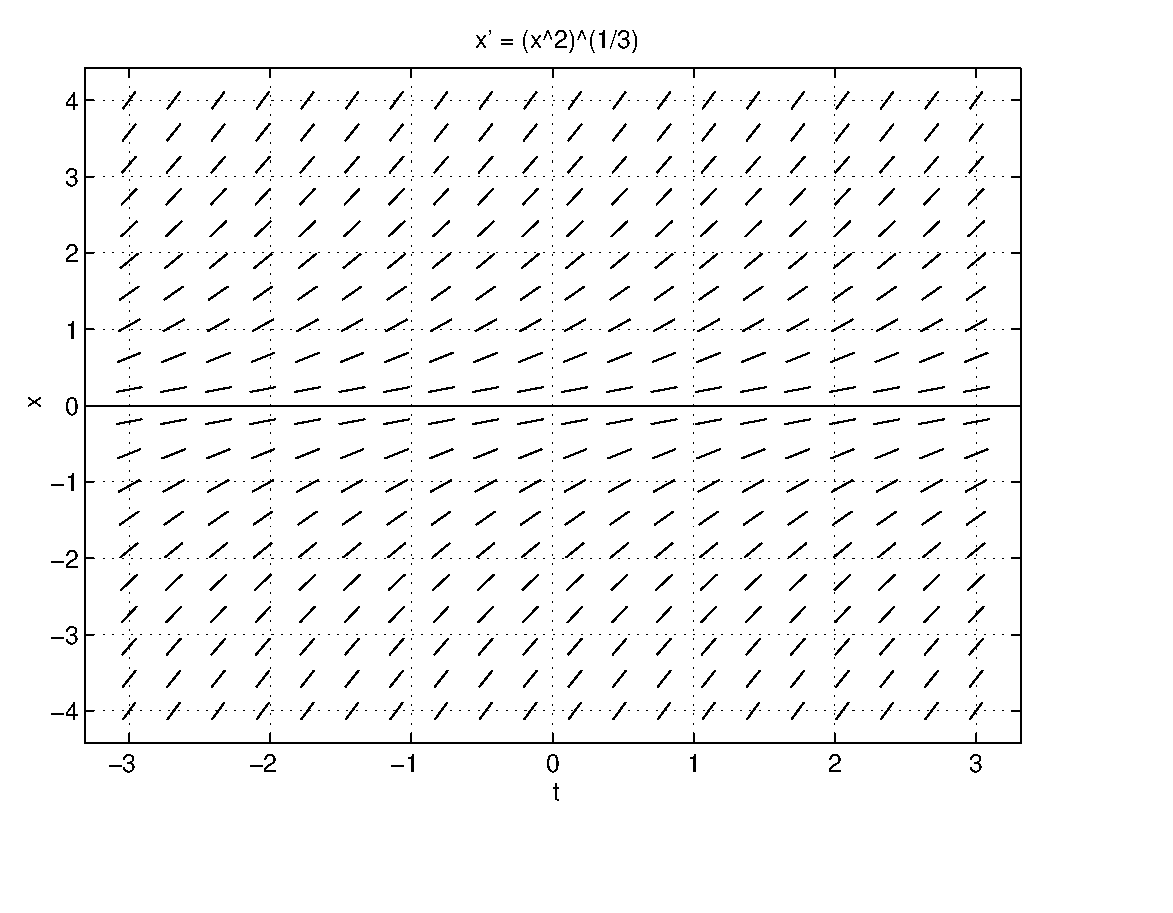
\psfig{file=../figures/nonuniqa.eps,width=3.2in}
	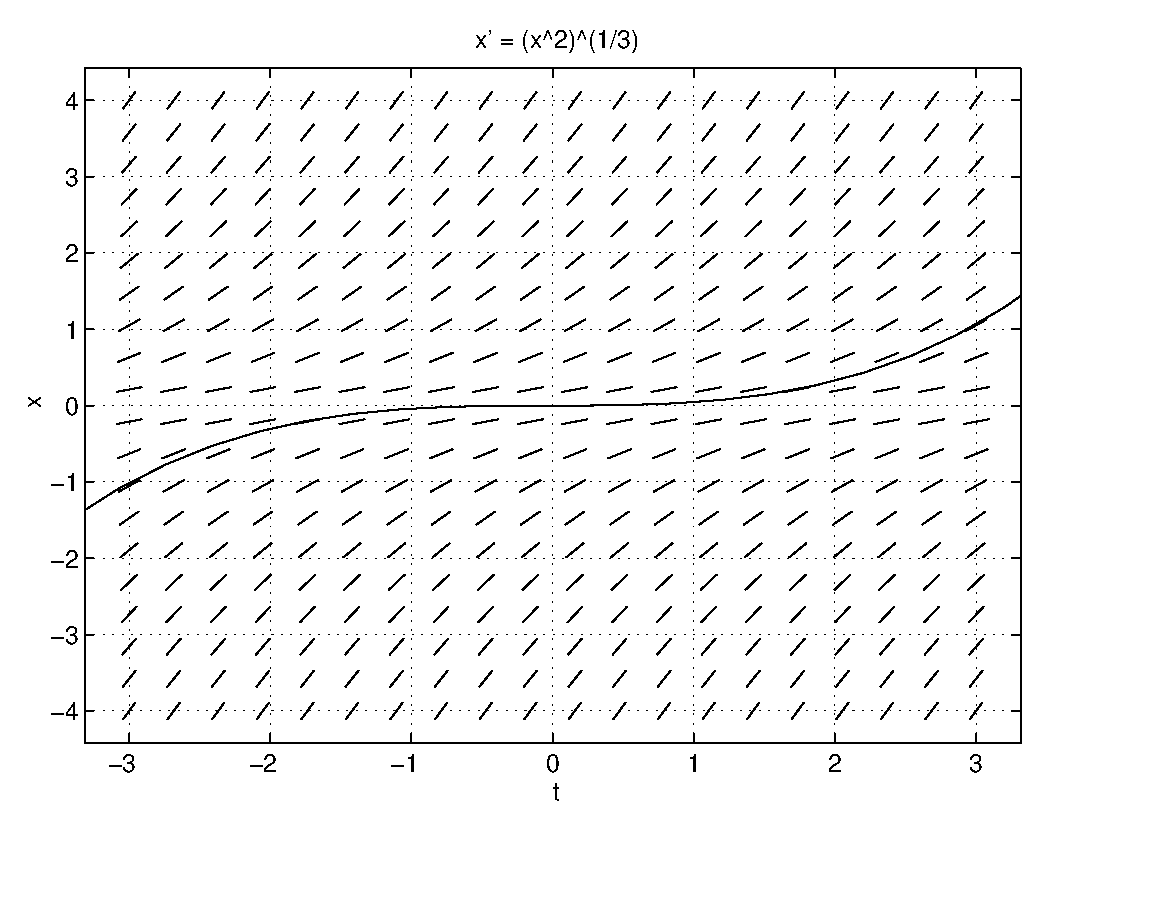
\psfig{file=../figures/nonuniqb.eps,width=3.2in}}
        \caption{Solutions for \protect\Ref{nonunique}
              for $t\in [-3,3]$ and $x\in [-4,4]$. Left: $x(0)=0$.
	      Right: $x(0)=0.00001$.}
        \label{nonuniquefig}
\end{figure*}

At this stage, we do not have the background to discuss the numerical
method employed by {\sf dfield5}.

\subsection*{The Initial Value Problem for Linear Systems}
\index{initial value problem}

In this chapter we discuss how to find solutions $(x(t),y(t))$ to
\Ref{2dlinsystem} satisfying the initial values $x(0)=x_0$ and $y(0)=y_0$.
It is convenient to rewrite \Ref{2dlinsystem} in matrix form as:
\begin{equation} \label{ndlinsystem}
\frac{dX}{dt}(t) = CX(t).
\end{equation}
The initial value problem is then stated as:  Find a solution to
\Ref{ndlinsystem} satisfying $X(0)=X_0$ where $X_0=(x_0,y_0)^t$.
Everything that we have said here works equally well for $n$
dimensional systems of linear differential equations.  Just let
$C$ be an $n\times n$ matrix and let $X_0$ be an $n$ vector
of initial conditions.

\subsubsection*{Solving the Initial Value Problem Using Superposition}

In Section~\ref{S:IVPR} we discussed how to solve~\Ref{ndlinsystem} when the
eigenvalues of $C$ are real and distinct.  Recall that when $\lambda_1$ and
$\lambda_2$ are distinct real eigenvalues of $C$ with associated
eigenvectors $v_1$ and $v_2$, there are two solutions to \Ref{ndlinsystem}
given by the explicit formulas
\[
X_1(t) = e^{\lambda_1 t}v_1 \AND X_2(t) = e^{\lambda_2 t}v_2.
\]
Superposition guarantees that every linear combination of these solutions
\[
X(t) = \alpha_1X_1(t)+\alpha_2X_2(t) =
\alpha_1e^{\lambda_1 t}v_1 + \alpha_2e^{\lambda_2 t}v_2
\]
is a solution to \Ref{ndlinsystem}.  In addition, we can always choose
scalars $\alpha_1,\alpha_2\in\R$ to solve any given initial value problem
of \Ref{ndlinsystem}.   It follows from the uniqueness of solutions to
initial value problems stated in Theorem~\ref{exist&unique} that all
solutions to \Ref{ndlinsystem} are included in this family of solutions.

We generalize this discussion so that we will be able to find closed form 
solutions to \Ref{ndlinsystem} in Section~\ref{S:TDM} when the eigenvalues 
of $C$ are complex or are real and equal.

Suppose that $X_1(t)$ and $X_2(t)$ are two solutions to \Ref{2dlinsystem} such
that
\[
v_1=X_1(0) \AND v_2=X_2(0)
\]
are linearly independent\index{linearly!independent}.  The existence part of
Theorem~\ref{exist&unique}
guarantees that such solutions exist.  Then all solutions to \Ref{2dlinsystem}
are linear combinations of these two solutions.  We verify this statement as
follows.  Corollary~\ref{C:dim=n} of Chapter~\ref{C:vectorspaces} states
that since $\{v_1,v_2\}$ is a linearly independent set in $\R^2$, it is
also a basis of $\R^2$.  Thus for every $X_0\in\R^2$ there exist scalars
$r_1,r_2$ such that
\[
X_0 = r_1v_1 + r_2v_2.
\]
It follows from superposition and Theorem~\ref{exist&unique} that the
solution
\[
X(t) = r_1X_1(t) + r_2X_2(t)
\]
is the unique solution whose initial condition vector is $X_0$.

We have proved that every solution to this linear system of differential
equations is a linear combination of these two solutions --- that is, we
have proved that the dimension of the space of solutions to \Ref{ndlinsystem}
is two.  This proof generalizes immediately to a proof of the following
theorem for $n\times n$ systems.

\begin{theorem}  \label{T:solvends}
Let $C$ be an $n\times n$ matrix.  Suppose that $X_1(t),\ldots,X_n(t)$
are  solutions to $\dot{X}=CX$ such that the vectors of initial conditions
$v_j=X_j(0)$ are linearly independent in $\R^n$.  Then the unique solution
to the system \Ref{ndlinsystem} with initial condition $X(0)=X_0$ is
\begin{equation}  \label{E:genlsoln}
X(t)=r_1X_1(t) + \cdots + r_nX_n(t),
\end{equation}
where $r_1,\ldots,r_n$ are scalars satisfying
\begin{equation} \label{findscalars}
X_0 = r_1v_1 + \cdots + r_nv_n.
\end{equation}
\end{theorem}\index{initial condition!linear independence}

We call \Ref{E:genlsoln} the {\em general solution\/} \index{general solution}
to the system of differential equations $\dot{X}=CX$.  When solving the
initial value problem we find a {\em particular solution\/}\index{particular
solution}
by specifying the scalars $r_1,\ldots,r_n$.

\begin{corollary}  \label{C:indsoln}
Let $C$ be an $n\times n$ matrix and let ${\cal X}=\{X_1(t),\ldots,X_n(t)\}$
be solutions to the differential equation $\dot{X}=CX$ such that the vectors
$X_j(0)$ are linearly independent in $\R^n$.  Then the set of all solutions
to $\dot{X}=CX$ is an $n$-dimensional subspace of $(\CCone)^n$, and
${\cal X}$ is a basis for the solution subspace.
\end{corollary}\index{subspace!of solutions}

Consider a special case of Theorem~\ref{T:solvends}.  Suppose that the
matrix $C$ has $n$ linearly independent eigenvectors $v_1,\ldots,v_n$ with
real eigenvalues $\lambda_1,\ldots,\lambda_n$.  Then the functions
$X_j(t)=e^{\lambda_j t}v_j$ are solutions to $\dot{X}=CX$.
Corollary~\ref{C:indsoln} implies that the functions $X_j$ form a basis for
the space of solutions of this system of differential equations.  Indeed,
the general solution to \Ref{ndlinsystem} is
\begin{equation}  \label{e:gensoln}
X(t) = r_1e^{\lambda_1 t}v_1 + \cdots + r_ne^{\lambda_n t}v_n.
\end{equation}
The particular solution that solves the initial value $X(0)=X_0$ is found by
solving \Ref{findscalars} for the scalars $r_1,\ldots,r_n$.





\EXER

\TEXER

\noindent In Exercises~\ref{c6.1.03a} -- \ref{c6.1.03d}, consider the system of
differential equations
\begin{equation} \label{Ex.1.03}
\begin{array}{rcr}
\frac{dx}{dt}  & = & 65x+42y \\
\frac{dy}{dt}  & = & -99x-64y.
\end{array}
\end{equation}
\begin{exercise} \label{c6.1.03a}
Verify that
\[
v_1 = \vectwo{2}{-3} \AND v_2 = \vectwo{-7}{11}
\]
are eigenvectors of the coefficient matrix of \Ref{Ex.1.03} and find
the associated eigenvalues.
\end{exercise}
\begin{exercise} \label{c6.1.03b}
Find the solution to \Ref{Ex.1.03} satisfying initial conditions $X(0) =
(-14,22)^t$.
\end{exercise}
\begin{exercise} \label{c6.1.03c}
Find the solution to \Ref{Ex.1.03} satisfying initial conditions $X(0) =
(-3,5)^t$.
\end{exercise}
\begin{exercise} \label{c6.1.03d}
Find the solution to \Ref{Ex.1.03} satisfying initial conditions $X(0) =
(9,-14)^t$.
\end{exercise}

\noindent In Exercises~\ref{c6.1.06a} -- \ref{c6.1.06d}, consider the system of
differential equations
\begin{equation} \label{Ex.1.06}
\begin{array}{rcr}
\frac{dx}{dt}  & = & x-y \\
\frac{dy}{dt}  & = & -x+y.
\end{array}
\end{equation}
\begin{exercise} \label{c6.1.06a}
The eigenvalues of the coefficient matrix of \Ref{Ex.1.06} are $0$ and $2$.
Find the associated eigenvectors.
\end{exercise}
\begin{exercise} \label{c6.1.06b}
Find the solution to \Ref{Ex.1.06} satisfying initial conditions
$X(0)=(2,-2)^t$.
\end{exercise}
\begin{exercise} \label{c6.1.06c}
Find the solution to \Ref{Ex.1.06} satisfying initial conditions
$X(0)=(2,6)^t$.
\end{exercise}
\begin{exercise} \label{c6.1.06d}
Find the solution to \Ref{Ex.1.06} satisfying initial conditions
$X(0)=(1,0)^t$.
\end{exercise}


\noindent In Exercises~\ref{c6.1.1a} -- \ref{c6.1.1d}, consider the system of
differential equations
\begin{equation} \label{E:c6.1.1}
\begin{array}{rcr}
\frac{dx}{dt}  & = & -y \\
\frac{dy}{dt}  & = &  x.
\end{array}
\end{equation}
\begin{exercise} \label{c6.1.1a}
Show that $(x_1(t),y_1(t)) = (\cos t,\sin t)$ is a solution to \Ref{E:c6.1.1}.
\end{exercise}
\begin{exercise} \label{c6.1.1b}
Show that $(x_2(t),y_2(t)) = (-\sin t,\cos t)$ is a solution to \Ref{E:c6.1.1}.
\end{exercise}
\begin{exercise} \label{c6.1.1c}
Using Exercises~\ref{c6.1.1a} and \ref{c6.1.1b}, find a solution $(x(t),y(t))$
to \Ref{E:c6.1.1} that satisfies $(x(0),y(0)) = (0,1)$.
\end{exercise}
\begin{exercise} \label{c6.1.1d}
Using Exercises~\ref{c6.1.1a} and \ref{c6.1.1b}, find a solution $(x(t),y(t))$
to \Ref{E:c6.1.1} that satisfies $(x(0),y(0)) = (1,1)$.
\end{exercise}

\noindent In Exercises~\ref{c6.1.2a} -- \ref{c6.1.2b}, consider the system of
differential equations
\begin{equation}  \label{E:c6.1.2}
\begin{array}{rcl}
\frac{dx}{dt} & = & -2x+7y \\
\frac{dy}{dt} & = &  5y,
\end{array}
\end{equation}
\begin{exercise} \label{c6.1.2a}
Find a solution to \Ref{E:c6.1.2}
satisfying the initial condition $(x(0),y(0)) = (1,0)$.
\end{exercise}
\begin{exercise} \label{c6.1.2b}
Find a solution to \Ref{E:c6.1.2}
satisfying the initial condition $(x(0),y(0)) = (-1,2)$.
\end{exercise}

\noindent In Exercises~\ref{c6.1.3a} -- \ref{c6.1.3c}, consider the matrix
\[
C = \left(\begin{array}{rrr} -1 & -10 & -6\\  0 & 4  & 3 \\  0  & -14  & -9
	\end{array}\right).
\]
\begin{exercise} \label{c6.1.3a}
Verify that
\[
v_1 = \left(\begin{array}{r} 1 \\ 0\\ 0\end{array}\right) \qquad
v_2 = \left(\begin{array}{r} 2 \\ -1\\ 2\end{array}\right) \quad \AND \quad
v_3 = \left(\begin{array}{r} 6 \\ -3\\ 7\end{array}\right)
\]
are eigenvectors of $C$ and find the associated eigenvalues.
\end{exercise}
\begin{exercise} \label{c6.1.3b}
Find a solution to the system of differential equations
$\dot{X}=CX$ satisfying the initial condition $X(0)= (10, -4, 9)^t$.
\end{exercise}
\begin{exercise} \label{c6.1.3c}
Find a solution to the system of differential equations
$\dot{X}=CX$ satisfying the initial condition $X(0)= ( 2, -1, 3)^t$.
\end{exercise}

\begin{exercise}  \label{c6.1.4A}
Show that for some nonzero $a$ the function $x(t)=at^5$ is a solution to the
differential equation $\dot{x}=x^{4/5}$.  Then show that there are at least
two solutions to the initial value problem $x(0)=0$ for this differential
equation.
\end{exercise}


\CEXER

\begin{exercise} \label{c6.1.4}
Use {\sf pplane5}\index{\computer!pplane5} to investigate the system
of differential equations
\begin{equation}  \label{Ex.1.4}
\begin{array}{rcr}
\frac{dx}{dt}  & = & -2y \\
\frac{dy}{dt}  & = &  -x+y.
\end{array}
\end{equation}
\begin{itemize}
\item[(a)] Use {\sf pplane5} to find two independent eigendirections (and
hence eigenvectors) for \Ref{Ex.1.4}.
\item[(b)] Using (a), find the eigenvalues of the coefficient matrix of
\Ref{Ex.1.4}.
\item[(c)] Find a closed form solution to \Ref{Ex.1.4} satisfying the initial
condition
\[
X(0) = \vectwo{4}{-1}.
\]
\item[(d)] Study the time series of $y$ versus $t$ for the solution in (c)
by comparing the graph of the closed form solution obtained in (c) with the
time series graph using {\sf pplane5}.
\end{itemize}
\end{exercise}




\end{document}
